\chapter{Results and discussion}\label{sec:results}
This chapter will review what has been done and
mentions the main open questions.
\par
Results using different tools
\par
limitations
\par
improvement (in relation to limitations)
%
\section{Results}
%
Tests has been performed to show the utility of the work done. The results are presented below. The testings are comparaisons between the results obtained with the previous workflow and the new one. The results obtained will then be reviewed by a specialist to evaluate the previous and the new segmented datasets.
%
\subsection{Bias correction}
%
Here we get going with the intensities inhomogeinities correction.
%
\subsubsection{Testing process}
%
we create a mask.
%
\begin{figure}\centering
\includegraphics[width=1\textwidth]{Images/Screenshots/BiasCorrection.png}
  \caption{Module created for the bias correction.% On the left panel, there are the parametersto set for the correction. On the top left red box, the 2d mask is displayed. On the top right box, the 3d mask is shown. On the lower left yellow slice, the biased volume is presented. In the lower right slice, the corrected volume is printed
  }\label{fig:BiasCorrection}
\end{figure}

%
\subsubsection{Results}
%
Here are the resultsfdd ddddddddddd dddddddddddd ddddddddddd ddddddddd dddddddddd ddddddddddd dddddddddd dddddddddd ddddddddd dddddddddd ddddddddd dddddddd dddddddd dddddd dddd dddddddd..
%
\par
\begin{figure}\centering
\begin{minipage}[c]{.45\textwidth}\centering
  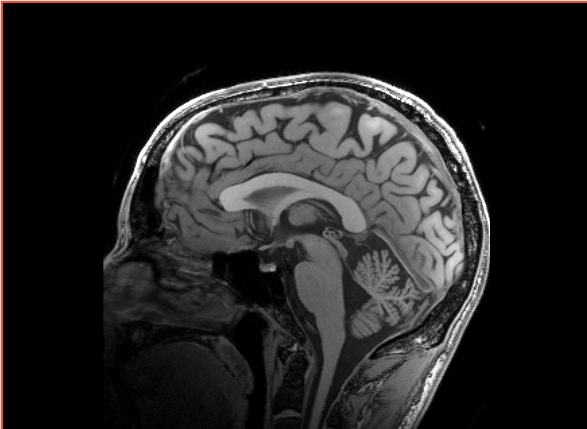
\includegraphics[width=.95\textwidth]{Images/Screenshots/T1SagittalNotCorrected.png}
  \caption{Sagittal view of a biased T1 volume.}\label{fig:T1SagittalNotCorrected}
\end{minipage}\hfill
\begin{minipage}[c]{.45\textwidth}\centering
  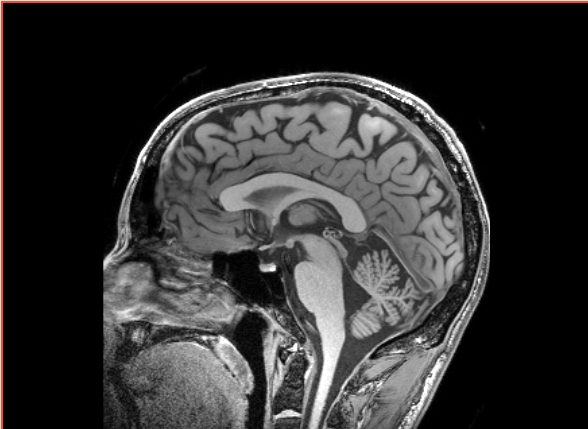
\includegraphics[width=.95\textwidth]{Images/Screenshots/T1SagittalCorrected.png}
  \caption{Sagittal view of the T1 volume after bias correction.}\label{fig:T1SagittalCorrected}
\end{minipage}
\end{figure}
%
\par
more comments ttttttttttttttttttttt ttttttttttttt ttttttttttt tttttttttttt ttttttttttt ttttttttttt tttttttttttttt ttttttttttttt tttttttttttttt tttttttttttt ttttttttttttttt\\
%
\subsubsection{Specialist's point of view}
%
\subsection{Global Prior estimation}
%
\subsubsection{Testing process}
%
\subsubsection{Results}
%
\subsubsection{Specialist's point of view}
%
\subsection{Class Selection}
%
\subsubsection{Testing process}
%
\subsubsection{Results}
%
\subsubsection{Specialist's point of view}
%
\section{Limitations}

\section{Future work}
\newpage
\section*{Acknowledgements}
\addcontentsline{toc}{chapter}{\numberline{}Acknowledgements}
Ron Kikinis who gave me the opportunity to carry out my intersnship in the SPL.
Sylvain Jaume who supervises me during all my work.
Andryi, Daniel, Steve?

